\documentclass[12pt, a4paper, twoside, titlepage]{article}
\usepackage[left=3cm, right=3cm, top=2cm]{geometry}
\usepackage{amsmath,mathtools}
\usepackage{bbold}
\usepackage{parskip}
\usepackage{mathabx}
\usepackage{cleveref} %% use \cref instead of \ref or \eqref
%% Tabels
\usepackage{siunitx,booktabs}
\usepackage[table]{xcolor}
% TIKZ Packages
\usepackage{tikz}
\usepackage{ifthen}
\usetikzlibrary{calc}
\usepackage{xcolor}
\usetikzlibrary{decorations.pathmorphing}
\usetikzlibrary{decorations.markings}

%% physics
\renewcommand{\H}{\ensuremath{\mathcal{H}}}
\newcommand{\ket}[1]{\ensuremath{\left|#1\right\rangle}}
\newcommand{\bra}[1]{\ensuremath{\left\langle#1\right|}}
\newcommand{\M}[1]{\ensuremath{\mathcal{M}_{\rm #1}}}
\newcommand{\Pp}[1]{\ensuremath{\mathbb{P}^{+}_{#1}}}
\newcommand{\Pm}[1]{\ensuremath{\mathbb{P}^{-}_{#1}}}
\begin{document}
\noindent \Large {\textbf{Tensor Study of Quantum Link Model}}
\normalsize
\\[2ex]
P. Stornati, P. Krah, D. Banerjee
\\[1ex]
Date: \today
\\[1ex]
\hrule$~$
  \\[2ex]


% \date{\today} date coulde be today
% \date{25.12.00} or be a certain date
% \date{ } or there is no date
% Hint: \title{what ever}, \author{who care} and \date{when ever} could stand
% before or after the \begin{document} command
% BUT the \maketitle command MUST come AFTER the \begin{document} command!
%\maketitle

%\tableofcontents % create a table of contens

%\newpage


\section{Hamiltonian of QLM as a spin system}

We want to study the Square Ice Hamiltonian
\begin{equation}
    \H = \sum_\square (-f_\square + \lambda f^2_\square)\,,\label{eq:hamiltonian}
\end{equation}
as the sum over all plaquettes:
\begin{equation}\label{eq:plaquette}
       f_\square = \sigma^+_{\mu_1}\sigma^+_{\mu_2}\sigma^-_{\mu_3}\sigma^-_{\mu_4}\, +  \sigma^-_{\mu_1}\sigma^-_{\mu_2}\sigma^+_{\mu_3}\sigma^+_{\mu_4}.
\end{equation}
on a long cylindrical lattice
\begin{align}\label{eq:geometry}
\Omega=\{\mu = (n,m) |\, n\in\{1,\dots,L_x\}, \;  m \in\{1,\dots L_y\}\}
\end{align}
displayed in \cref{fig:lattice}.
\begin{figure}[hp!]
  

\colorlet{colP1}{gray!60}
\colorlet{colP2}{gray!20}
\colorlet{actcol}{blue!60}



\begin{tikzpicture}[scale=1.6]
	
 % ================================================================  
 % Spatial
  % ================================================================  	
	\coordinate (A) at (0,0);
	\coordinate (B) at (7,2);
	\fill[colP2,thick] (A) rectangle (B);
	
	\coordinate (P1a) at (2.5,8.5);
	\coordinate (P1b) at (8.5,2.5);
	\coordinate (P2a) at (P1b);
	\coordinate (P2b) at (10,1);
	\coordinate (P3a) at (P1b);
	\coordinate (P3b) at (10,8.5);
	\coordinate (P4a) at (2.5,2.5);
	\coordinate (P4b) at (8.5,10);
	
	\coordinate (P5a) at (2.5,2.5);
	\coordinate (P5b) at (1,1);
	\coordinate (P6a) at (P1a);
	\coordinate (P6b) at (1,10);
	\coordinate (P4a) at (P3b);
	\coordinate (P4b) at (8.5,10);
	
	
	%\fill[dashed,colP1,thick] (P1a) rectangle (P1b);
	
	%\fill[dashed,colP1,thick] (P2a) rectangle (P2b);	
	
	%\fill[dashed,colP2,thick] (P3a) rectangle (P3b);	
	
	%\fill[dashed,colP1,thick] (P4a) rectangle (P4b);	
	
	%\fill[dashed,colP1,thick] (P5a) rectangle (P5b);	
	
	%\fill[dashed,colP1,thick] (P6a) rectangle (P6b);	

	 %% ----------------------------------------  
	 %%grid
	%\draw[step=2cm,black!60,thick] (0,0) grid (12,4);
	 % ----------------------------------------  
	 % boundary links
	  % ----------------------------------------  
        
        \draw[actcol, decorate, decoration=zigzag] (-1, 0) -- (-0.2,0) node [pos=0.66,below] {};
        \draw[-] (-1, 0) -- (-0.2,0) node [pos=0.66,below] {};
        \draw[actcol, decorate, decoration=zigzag] (-1, 1) -- (-0.2,1) node [pos=0.66,below] {};
        \draw[-] (-1, 1) -- (-0.2,1) node [pos=0.66,below] {};
        \draw[actcol, decorate, decoration=zigzag] (7, 1) -- (8,1) node [pos=0.66,below] {};
        \draw[actcol, decorate, decoration=zigzag] (7, 0) -- (8,0) node [pos=0.66,below] {};
        \draw[dashed] (-1, 2) -- (-0.2,2) node [pos=0.66,below] {};

        \newcounter{ga}\setcounter{ga}{0}
	\foreach \x in {0,1,...,7} 
	{	
		\foreach \y in {0,1,...,2} 
		{		
	        	  \ifthenelse{\x<8 \AND \y<2}
                         {
                          \stepcounter{ga}
                        \draw[-] (\x,\y ) -- (\x+0.9,\y) node [pos=0.5,below] {$\sigma_{\thega}$};
                          \stepcounter{ga}
                          \draw[-] (\x,\y ) -- (\x,\y+0.9) node [pos=0.5,left] {$\sigma_{\thega}$};
	         	}{
                            \draw[dashed] (\x,\y ) -- (\x,\y+0.9) node [pos=0.66,below] {};
                            \draw[dashed] (\x,\y ) -- (\x+0.9,\y) node [pos=0.66,below] {};
                          }
				
				
                          %\fill (\x+0.5,\y+0.5)  circle[radius=1.5pt] node [anchor=south west] {(\x,\y)};
                          \fill (\x,\y)  circle[radius=1.5pt] node [anchor=south west] {(\x,\y)};
					

				
		}	
	}	
	
	
	 % ----------------------------------------  
        \draw[->] (-1,-1 ) -- (-0.5,-1) node [pos=0.66,below] {$\hat{x}$};
      \draw[->] (-1, -1 ) -- (-1, -0.5) node [pos=0.66,left] {$\hat{y}$};
 
        %%%%%%%%%%%%%%%%%%%
        % Legend
        %%%%%%%%%%%%%%%%%%
        \draw[actcol, decorate, decoration=zigzag] (5,-0.7 ) -- (5.5,-0.7) node [pos=0.66,below] {};
        \draw[-] (5,-0.7 ) -- (5.5,-0.7) node [pos=1.66,right] {fixed link};
        \draw[-] (2.5,-0.7 ) -- (3,-0.7) node [pos=1.66,right] {link};
        \draw[dashed] (2.5,-1 ) -- (3,-1) node [pos=1.66,right] {periodic link};
        \fill[colP2,thick] (5,-0.9) rectangle (5.5,-1.1);
        \node [fill=white] at (5.8,-1) [right] {domain $\Omega$};
	 
	 
\end{tikzpicture}



  \caption{Definition of the computational mesh}
  \label{fig:lattice}
\end{figure}

In the conventional up/down $s^\pm\in\mathbb{R}^2$ ([1 0]/[0 1]) basis the  link operators
$\sigma^{\pm}$ are pauli matrices :
\begin{align}
\sigma^+=
\begin{pmatrix}
0 & 1 \\
0 & 0
\end{pmatrix}
\quad
\sigma^-=
\begin{pmatrix}
0 & 0 \\
1 & 0
\end{pmatrix}
\qquad
I_2 =
\begin{pmatrix}
1 & 0 \\
0 & 1
\end{pmatrix}
\end{align}


In all our lattices $L_y \ll L_x$. For now we fix $L_y = 2$ as in \cref{fig:lattice}.
Before explaining the computations we want to point out some properties of the Hamiltonian.

%%%%%%%%%%%%%%%%%%%%%%%%%%%%%%%%%%%%%%%%%%%%%%%%%%%%%%%%%%%%%%%%%%%%%%%%%%%%%%%%%%%%
\subsection{Mathematical Properties of the Quantum Link Model}
%%%%%%%%%%%%%%%%%%%%%%%%%%%%%%%%%%%%%%%%%%%%%%%%%%%%%%%%%%%%%%%%%%%%%%%%%%%%%%%%%%%%
\paragraph{Gauss Law:}
The Hamiltonian \H\, in \cref{eq:hamiltonian}
commutes with the \textit{vertex operator} $G_\mu$, which counts the number of in and
outgoing arrows at vertex $\mu$. We can therefore fix the total charge at each vertex
with the \textit{Gauss law constraint}:
\begin{align}\label{eq:ice_rule}
  G_\mu&=0 \qquad\text{ for all }\qquad \mu \in \Omega\,,\\
  G_\mu &\coloneqq \sum_{\hat{i}\in\{\hat{x},\hat{y}\}} ( s_{\nu-\hat{i}/2}-s_{\nu+\hat{i}/2})\,.
\end{align}
\paragraph{Winding Numbers}
\begin{equation}
  W_y = \frac{1}{2L_y}\sum_\mu E_{\mu,x}
\end{equation}
\paragraph{Fluxes}
\subsection{Hilbert-Space}
In the absence of the ice rule eq.\eqref{eq:ice_rule} the hilbertspace becomes $2^{2\cdot L_xL_y}$ dimensional  and the linear combination of every state is given by:
\begin{equation}\label{eq:hilbertspace}
|\psi\rangle = \sum_{i_1,i_2,\dots,i_{L_x}}A_{i_1,i_2,\dots,i_{L_x}} \,|i_1\rangle|i_2\rangle\dots|i_{L_x}\rangle
\end{equation}
where $i_n=1,2,\dots,2^{2L_y}$ labels the corresponding quantum state at site $n$. For the $L_y=2$
we thus have 16 different quantum states at each site $|i_n\rangle=|(s_1,s_2,s_3,s_4)\rangle$,
where $s_i\in\{0,1\}$ labels the $i$th spin in the local basis drawn in \cref{fig:locbasis}.
The 16 different combinations in the set can be explicitly written down:
\begin{equation}
  %
  \left \{
  \begin{pmatrix}
  1  \\
  1 \\
  1 \\
  1 \\
  \end{pmatrix},
  %
  %
  \begin{pmatrix}
  1  \\
  0 \\
  1 \\
  1 \\
  \end{pmatrix},
  %
  %
  \begin{pmatrix}
  1  \\
  1 \\
  0 \\
  1 \\
  \end{pmatrix},
%
  \begin{pmatrix}
  1  \\
  1 \\
  1 \\
  0 \\
  \end{pmatrix},
  %
%
  \begin{pmatrix}
  0  \\
  0 \\
  1 \\
  1 \\
  \end{pmatrix},
 %
  \cdots,
  \begin{pmatrix}
  0  \\
  0 \\
  0 \\
  1 \\
  \end{pmatrix},
  %%
  \begin{pmatrix}
  0  \\
  0 \\
  0 \\
  0 \\
  \end{pmatrix}
  % %
  \right\}
  %
\end{equation}
The number of elements in the set will be also referred to as local hilbertspace dimension $D$.

\newpage
\section{Computational Basis}
For the MPS we have to rewrite the Hamiltonian of the system in the nearest neighbour setting.
The local Hamiltonian $H_{n,n+1}$ thus defines the interaction between the states at site
$|i_n\rangle$ and $|i_{n+1}\rangle$.
The Hamilton operator \eqref{eq:hamiltonian} consists of 4 terms.
Where on each site we have $m=1,\dots,L_y$ possible interactions.
Thus the hamiltonian consists of $4L_y$ Kronecker products:
\begin{align}
H_{n,n+1}= \sum_{j=1}^4\sum_{m=1}^{L_y}h^{(j)}_{\sqsubset,n,m} \otimes h^{(j)}_{\sqsupset,n+1,m}\label{eq:Hloc}
\end{align}

\begin{figure}[hp!]
  \centering
  % 2. Local basis
\colorlet{colP2}{gray!20}
\begin{tikzpicture}[scale=1.6]
	
 % ================================================================  
 % Spatial
  % ================================================================  	
	\coordinate (A) at (0,0);
	\coordinate (B) at (1,2);
	\fill[colP2,thick] (A) rectangle (B);
	\fill[colP2,thick] (4,0) rectangle (5,2);
	

        % title
        \node [fill=white] at (0.5,2.2) {left local basis};
        % horizontal links
        \draw[-] (0,0 ) -- (0.9,0) node [pos=0.5,below] {$s^l_{1}$};
        \draw[-] (0,1 ) -- (0.9,1) node [pos=0.5,below] {$s^l_{3}$};
        \draw[dashed] (0,2 ) -- (0.9,2) node [pos=0.5,below] {};
        %vertical links
        \draw[-] (0,0 ) -- (0,0.9) node [pos=0.5,left] {$s^l_{2}$};
        \draw[-] (0,1 ) -- (0,1.9) node [pos=0.5,left] {$s^l_{4}$};
        \fill (0,0)  circle[radius=1.5pt] node [anchor=south west] {(n,0)};
        \fill (0,1)  circle[radius=1.5pt] node [anchor=south west] {(n,1)};
        \fill[black!40] (1,0)  circle[radius=1.5pt] node [anchor=south west] {(n+1,0)};
        \fill[black!40] (1,1)  circle[radius=1.5pt] node [anchor=south west] {(n+1,1)};
        \fill[black!40] (0,2)  circle[radius=1.5pt] node [anchor=south west] {};
        \fill[black!40] (1,2)  circle[radius=1.5pt] node [anchor=south west] {};
                              
        %title
        \node [fill=white] at (4.5,2.2)  {right local basis};
         % horizontal links
        \draw[-] (4,0 ) -- (4.9,0) node [pos=0.5,below] {$s^r_{1}$};
        \draw[-] (4,1 ) -- (4.9,1) node [pos=0.5,below] {$s^r_{3}$};
        \draw[dashed] (4,2 ) -- (4.9,2) node [pos=0.5,below] {};
        %vertical links
        \draw[-] (5,0 ) -- (5,0.9) node [pos=0.5,left] {$s^r_{2}$};
        \draw[-] (5,1 ) -- (5,1.9) node [pos=0.5,left] {$s^r_{4}$};
        \fill (5,0)  circle[radius=1.5pt] node [anchor=south west] {(n+1,0)};
        \fill (5,1)  circle[radius=1.5pt] node [anchor=south west] {(n+1,1)};
        \fill[black!40] (4,0)  circle[radius=1.5pt] node [anchor=south east] {(n,0)};
        \fill[black!40] (4,1)  circle[radius=1.5pt] node [anchor=south east] {(n,1)};
        \fill[black!40] (5,2)  circle[radius=1.5pt] node [anchor=south west] {};
        \fill[black!40] (4,2)  circle[radius=1.5pt] node [anchor=south west] {};
                              
                                      

                              
	
	
	 % ----------------------------------------  
        
	 
\end{tikzpicture}

  \caption{Definition of the computational mesh}
  \label{fig:locbasis}
\end{figure}

To identify the different local interaction terms in the Hamilton operator  \eqref{eq:Hloc} with \eqref{eq:hamiltonian} we rewrite the
plaquette-operator into our computational basis $|i_n\rangle$. A plaquette operator defines our nearest neighbor interaction between state
$|i_n\rangle$ and $|i_{n+1}\rangle$
\begin{align}
f_\square &= f_{\sqsubset,n,m}\otimes f_{\sqsupset,n,m} + h.c.\\
f_{\sqsubset,n,m} &= \sigma^-_{r,n,m+1}\sigma^-_{v,n,m+1}\sigma^+_{r,n,m}\\
f_{\sqsupset,n+1,m} &= \sigma^+_{l,n+1,m+1}\sigma^+_{v,n+1,m+1}\sigma^-_{l,n+1,m}
\end{align}
Comparing this to \eqref{eq:Hloc} yields:
\begin{align}
h^{(1)}_{\sqsubset,n,m} &=- f_{\sqsubset,n,m}\quad
&h^{(1)}_{\sqsupset,n+1,m} = f_{\sqsupset,n+1,m}\\
%%%%
h^{(2)}_{\sqsubset,n,m} &=- f^\dagger_{\sqsubset,n,m}
\quad
&h^{(2)}_{\sqsupset,n+1,m} = f^\dagger_{\sqsupset,n+1,m}\\
%%%%
h^{(3)}_{\sqsubset,n,m} &=\lambda f^\dagger_{\sqsubset,n,m}f_{\sqsubset,n,m}
\quad
&h^{(3)}_{\sqsupset,n+1,m} = f^\dagger_{\sqsupset,n+1,m}f_{\sqsupset,n+1,m}\\
%%%%
h^{(4)}_{\sqsubset,n,m} &=
\lambda f_{\sqsubset,n,m}f^\dagger_{\sqsubset,n,m}
\quad
&h^{(4)}_{\sqsupset,n+1,m} =
f_{\sqsupset,n+1,m}f^\dagger_{\sqsupset,n+1,m}\\
\end{align}

For example in our $L_y=2$ system we get $64 \times 64$ size Operators :

\begin{align}
h^{(1)}_{\sqsubset,n,m} &=-\sigma^+\otimes\sigma^-\otimes\sigma^+\otimes I_2 \otimes I_2 \otimes I_2 \in \mathbb{R}^{2^6,2^6}\\
h^{(1)}_{\sqsupset,n,m} &=I_2 \otimes I_2 \otimes \sigma^+ \otimes I_2\otimes\sigma^-\otimes\sigma^+ \in \mathbb{R}^{2^6,2^6}\\
\end{align}
Note that this allready inherits the periodicity in $\hat{y}$. For the choosen up/down ([1 0]/[0 1]) basis the link operators are given by:
\begin{align}
\sigma^+=
\begin{pmatrix}
0 & 1 \\
0 & 0
\end{pmatrix}
\quad
\sigma^-=
\begin{pmatrix}
0 & 0 \\
1 & 0
\end{pmatrix}
\qquad
I_2 =
\begin{pmatrix}
1 & 0 \\
0 & 1
\end{pmatrix}
\end{align}





\begin{align}
	f^2_\square= \sigma^+_{\mu_1} \sigma^-_{\mu_1} \, \sigma^+_{\mu_2} \sigma^-_{\mu_2} \, \sigma^-_{\mu_3} \sigma^+_{\mu_3} \, \sigma^-_{\mu_4} \sigma^+_{\mu_4}  \, + hc
\end{align}

If we define $p+$ and $p+$ as:
\begin{align}
	p+= \frac{ \mathbb{1} + \sigma^z }{2} \; ;	\; p-= \frac{ \mathbb{1} - \sigma^z }{2}
\end{align}

I have:

\begin{equation}\label{eq:plaquette}
	f^2_\square = p^+_{\mu_1}p^+_{\mu_2} p^-_{\mu_3} p^-_{\mu_4}\, +  p^-_{\mu_1} p^-_{\mu_2} p^+_{\mu_3} p^+_{\mu_4}
\end{equation}

\subsection{Todos}
\begin{itemize}
  \item Hamiltonian in external magnetic field, $\phi_\square\in \mathbb{R}$.
    Therefore we define the generalized plaquette operator
    \begin{align}
      f(\phi_\square) \coloneqq u_\square e^{i\phi_\square}+ u^\dagger_\square e^{-i\phi_\square}
    \end{align}
    and plug it in \eqref{eq:hamiltonian}
  \item Winding number operators
    \begin{align}
      W_y =
    \end{align}
\end{itemize}

\section{Order Parameters}
 To detect the phase transitions, we study the so-called sublattice
 magnetization $( \M{A}, \M{B})$ which are defined as follows:
 \begin{align}
	 \M{A}(x) &= \Pp{x,\mu} \Pp{x+\mu,\nu} \Pm{x+\nu,\mu} \Pm{x,\nu} -
          \Pm{x,\mu} \Pm{x+\mu,\nu} \Pp{x+\nu,\mu} \Pp{x,\nu}
 \end{align}
 where $\Pp{x,\mu}$ and $\Pm{x,\mu}$ are the projection operators
 on the spin components $S^z = \pm \frac{1}{2}$ respectively.


%\end{thebibliography}
\newpage
\section{Numerical Results and Simulation Parameters}

\begin{table}[htp!]
\centering
\caption{Parameter sets for all Simulations}
\smallskip
\sisetup{table-format = 3.2}
\begin{tabular}{l l l}
\toprule
Parameters & \multicolumn{1}{l}{Simulation 1} & \multicolumn{1}{l}{Simulation 2} \\
\midrule
\rowcolor[gray]{.9}
Vertical grid size $L_x$ & {20,40,60,100,200} & 60\\
Horizontal grid size $L_y$           & 2 & 2 \\
\rowcolor[gray]{.9}
Coupling $\lambda$ & $[-4.0,-3.5,-3.0,\dots,-1.0]$ & -1.0\\
Magnetic field angle $\theta$       & 0 & $\theta_k =\frac{\pi}{4}k, k =\{ 0,1,\dots,8\}$ \\
\rowcolor[gray]{.9}
\bottomrule
\end{tabular}
\end{table}

\begin{figure}[htp!]
  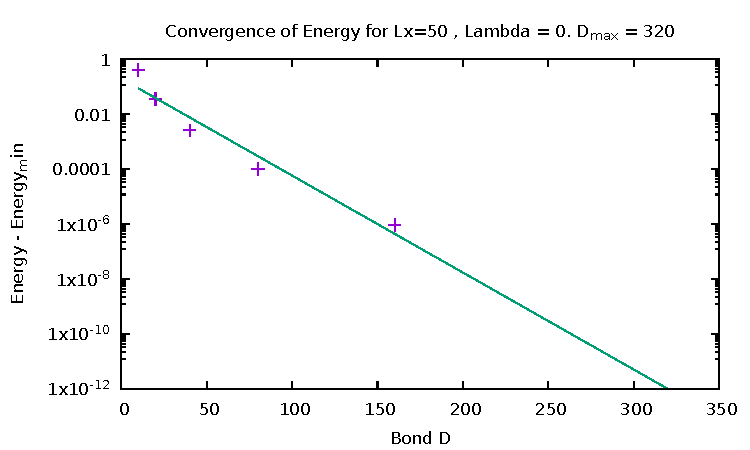
\includegraphics{../DMRG_QLM/data/extrapolation_in_bond_D/L_50/plot_extrapolation_in_bond_D_L_50_lam_0.pdf}
  \caption{Extrapolation of the bond dimension}
  \label{}
\end{figure}


\end{document}
